\chapter{Resultados y Evaluación}
\label{cap:resultadosyevaluacion}

Finalmente tranformando la información del data frame final en una gráfica con los sentimientos predominantes (Figura \ref{fig:most_frecuent_sentiments}) podemos observar que aunque si que haya asignado sentimientos a las letras de las canciones es un poco raro que haya tal cantidad de enfado en ellas. Para ello veamos más detenidamente los resultados de otros países.

\begin{figure}[h]
	\centering
	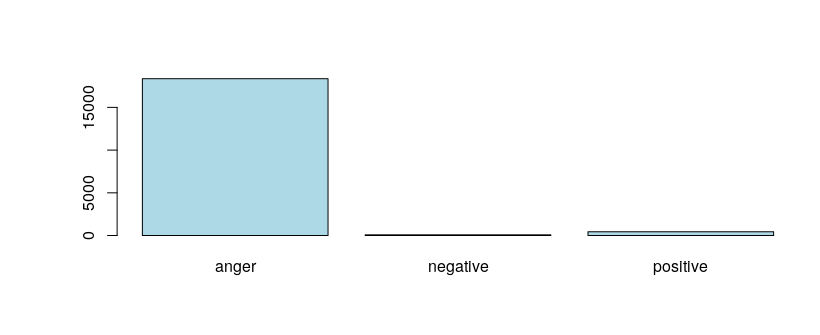
\includegraphics[width=\linewidth]{Imagenes/most_frecuent_sentiments}
	\caption{Principales sentimientos}
	\label{fig:most_frecuent_sentiments}
\end{figure}

Como podemos ver en las Figuras \ref{fig:country12}, \ref{fig:country2} y \ref{fig:country1}, en países de habla inglesa como Estados Unidos, Reino Unido o Australia, el reparto entre sentimientos positivos y de enfado es bastante equitativo. Sin embargo podemos observar que países en los que las letras no son en inglés o solo una pequeña parte son en inglés automáticamente el sentimiento es clasificado como de enfado. Se puede ver claramente en países como Colombia, Noruega, Tayikistán, etc...

\begin{figure}[h]
	\centering
	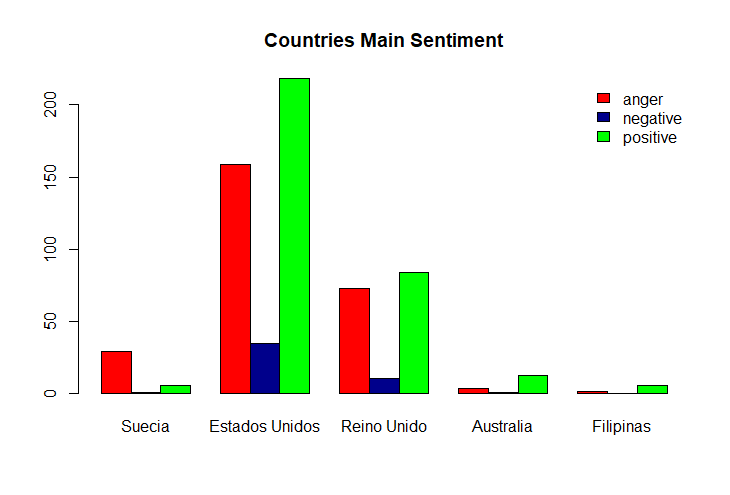
\includegraphics[width=\linewidth]{Imagenes/country12}
	\caption{Sentimientos detallados por paises}
	\label{fig:country12}
\end{figure}

\begin{figure}[h!]
	\centering
	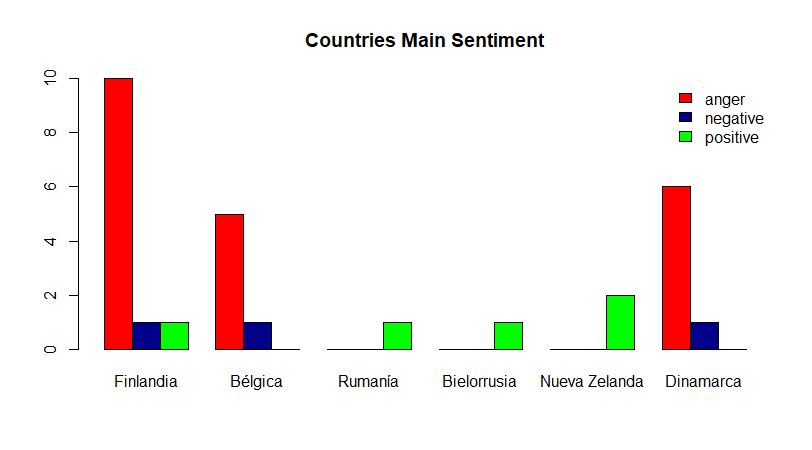
\includegraphics[width=\linewidth]{Imagenes/country2}
	\caption{Sentimientos detallados por paises}
	\label{fig:country2}
\end{figure}

\begin{figure}[h]
	\centering
	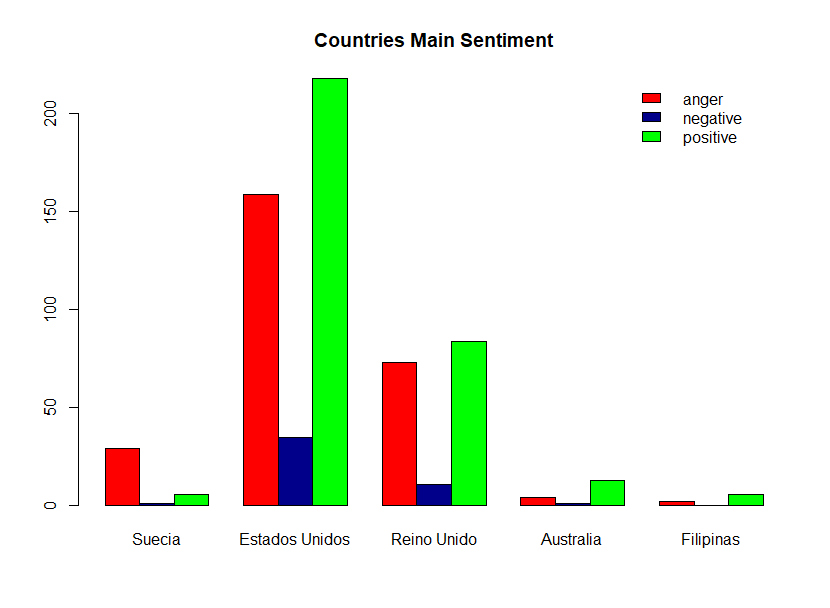
\includegraphics[width=\linewidth]{Imagenes/country1}
	\caption{Sentimientos detallados por paises}
	\label{fig:country1}
\end{figure}

\begin{figure}[h]
	\centering
	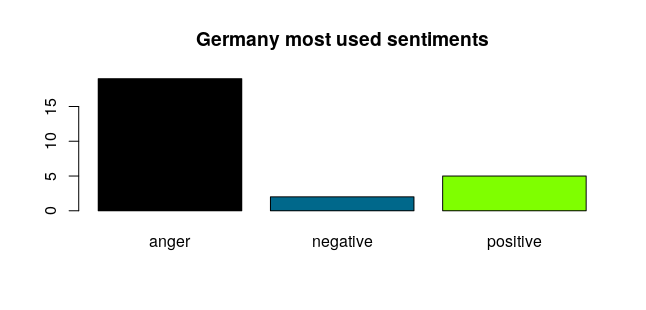
\includegraphics[width=0.7\linewidth]{Imagenes/Germany}
	\caption{Sentimientos detallados en Alemania}
	\label{fig:Germany}
\end{figure}

Por último si miramos la distribución en España en la Figura \ref{fig:SpainSentiments}, vemos que absolutamente todos los artistas han sido clasificados con un sentimiento de enfado. Una de los posibles fallos es que el diccionario de sentimientos en cuanto detecta otra palabra en otro idioma la clasifica automáticamente como dicho sentimiento, lo cual hace que esté tan presente.

\begin{figure}[h]
	\centering
	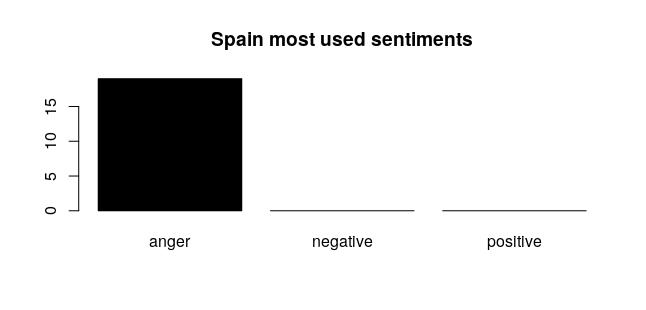
\includegraphics[width=0.7\linewidth]{Imagenes/SpainSentiments}
	\caption{Sentimientos detallados en España}
	\label{fig:SpainSentiments}
\end{figure}

Los resultados observados en la figura \ref{fig:SpainSentiments} indican de que otro de los mayores retos con los que nos hemos encontrado es la barrera del idioma. Dicho problema nos abre las puertas a continuar este trabajo y ampliarlo con nuevas técnicas de traducción e intrepretación de textos, lo cual lo veremos en el próximo Capítulo.